\chapter{Propuesta de trabajo de grado}

\section{Planteamiento del problema}
\setlength{\parskip}{5mm}


Actualmente al asistir a la cita para la inspección del vehículo, el perito registra las especificaciones del mismo en una hoja para luego ser archivada y guardada, este proceso se realiza manualmente.

El procesos presenta una serie de inconveniente en cuando a la persistencia de los datos y la administración se refiere:

\begin{itemize}

	\item Las planillas de inspección se guardan solamente en físico.

	\item El riesgo de perder información que no esta respaldada.

	\item El acceso a la información, al ser una búsqueda manual, no es eficiente. 

\end{itemize}


Ante la situación descrita, se plantea elaborar una solución con tecnología Web, que permita a los peritos, mantener un registro digital de las planillas de inspección de los vehículos.



% Recibirá mediante un web service la información de la planilla y que esta pueda ser editada una vez antes de aceptar y guardarla en el sistema

% Mantener este registro de forma sistematizada 

% Actualmente al asistir a la cita para la inspección del vehiculo, se anotan las especificaciones del mismo en una hoja para luego ser pasada a la computadora, este proceso ocasiona gastos de recursos tanto del personal encargado de traspasar la informacion  como insumos como hojas entre otras  

% Recibirá mediante un web service la información de la planilla y que esta pueda ser editada una vez antes de aceptar y guardarla en el sistema

\setlength{\parskip}{0mm}


% diagrama y arquitectura


\section{Justificación}


Un sistema con tecnologías web, es la mejor solución para sistematizar la administración de las planillas de inspección y para el almacenamiento de las mismas de forma digital, para que de esta forma la empresa aseguradora pueda llevar un registro cuyo gestión sea mas eficiente y de múltiple acceso.

La implementación de este sistema representa una reducción riesgos y costos a largo plazo para la compañía, permitiendo que la gestión de las planillas de inspección y los procesos vinculados con ellas se lleven acabo de manera óptima.


\section{Objetivo general}

% Desarrollar una aplicación con tecnología móvil multiplataforma y una aplicación con tecnología web, que permita sistematizar la planilla de inscripción para ser utilizada por el personal de una empresa de Seguros. 
Desarrollar una solución para el proceso de inspección de vehículos en una compañía de seguros.

\section{Objetivos específicos}

\begin{itemize}

	
	
	% \item Permitir la edición de la solicitudes de inscripción mediante la aplicación web.
	% \item Análisis y levantamiento de información.

	% \item Diseñar prototipos.

	% \item Diseñar la base de datos.

	% \item Diseñar interfaces de la aplicación web.

	% \item Implementar funcionalidades del sistema.
	% % \item Diseñar e implementar un sistema de registro.

   \item Análisis de especificaciones del proceso de inspección de vehículos para suscripción

   \item Diseño del modelo de datos, de las interfaces y de los componentes de los módulos del sistema

   \item Desarrollo del sistema

   \item Pruebas funcionales y de usabilidad
	
	

\end{itemize}



\subsection{Solución Propuesta}
\setlength{\parskip}{5mm}
Se propone el uso de un sistema web con la finalidad de mantener la persistencia de las planilla de registro del seguro digitalmente, y facilitar su acceso y edición de las mismas. Este sistema web estará compuesto de varios módulos, un modulo de registro donde el personal de la compañía encargado de la gestión de estas solicitudes podrá registrarse para tener acceso al segundo modulo que es el de edición y aprobación de las solicitudes de inscripción de la compañía de seguros.


%Para ello se propone el desarrollo de la siguiente arquitectura descrita:
%imagen computadora  -  servidor

\begin{figure}[H]
\begin{center}
	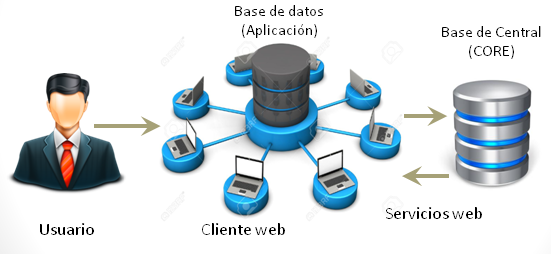
\includegraphics[width=15cm,height=7cm]{img/sin_tecnologia1.png}
\end{center}
\caption{Propuesta de solución conceptual.}
\label{fig:Sin_Tec}
\end{figure}

Esta arquitectura consiste básicamente en un cliente que realiza peticiones a otro programa (el servidor) que le da respuesta.

\begin{figure}[H]
\begin{center}
	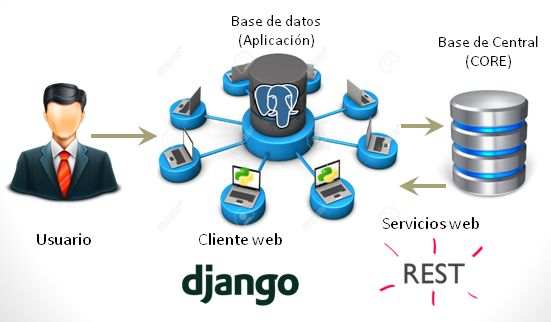
\includegraphics[width=15cm,height=7cm]{img/con_tecnologia1.png}
\end{center}
\caption{Propuesta de solución.}
\label{fig:Con_Tec}
\end{figure}

%Dentro de esta arquitectura se pretende utilizar las siguientes herramientas que se muestran a continuacion:
%imagen computadora  -  servidor con postgres y python
Para la base de datos utilizaremos PostgreSQL, ya que es una de las bases de datos mas potentes de software libre, con un alto rendimiento, seguridad y a su vez estar disponible prácticamente para todas las versiones de los sistemas operativos Unix y también Windows. Su versatilidad y robustez la hace el candidato perfecto para el sistema que se busca implementar.

Se propone utilizar el framework de Django para el desarrollo del sistema. Ya que siendo uno de los muchos frameworks que están establecidos sobre la base del patrón MVC en sus beneficios se encuentra la separación de responsabilidad y organización del código. Este framework incorpora un patrón llamado MTV (Modelo-Template-Vista), los templates son donde se implementan todas las interfaces de los usuarios, que serán desplegadas por las vistas en el lado del servidor y los models corresponde a la base da datos donde persistirá la información. Además posee un sistema jerárquico de plantilla que proporciona la reutilización de código y la extensibilidad de las aplicaciones. Posee un buen soporte para PostgresSQL, la base de datos que se piensa utilizar para el sistema. 

\setlength{\parskip}{0mm}


\newpage
\subsection{Metodología de desarrollo a utilizar}

\setlength{\parskip}{5mm}
Para el desarrollo de este proyecto, se quiere utilizar la metodología Scrum, ya que es una de las metodologías mas usadas actualmente en el mercado para la realización de proyectos. Esta metodología aplica de manera regular un conjunto de mejores prácticas para trabajar en equipo y obtener el mejor resultado posible de un proyecto.

Es esta metodología se realizan entregas parciales del resultado final del proyecto, priorizadas por el beneficio que aportan al receptor. Cada interacción permite evaluar el desempeño de las funcionalidades asociadas al sistema. Posee la flexibilidad y adaptación de trabajar respecto a las necesidades del cliente. 

\setlength{\parskip}{0mm}

\newpage
\section{Descripción del flujo asociado a la solución}

%Falta

\begin{figure}[H]
\begin{center}
	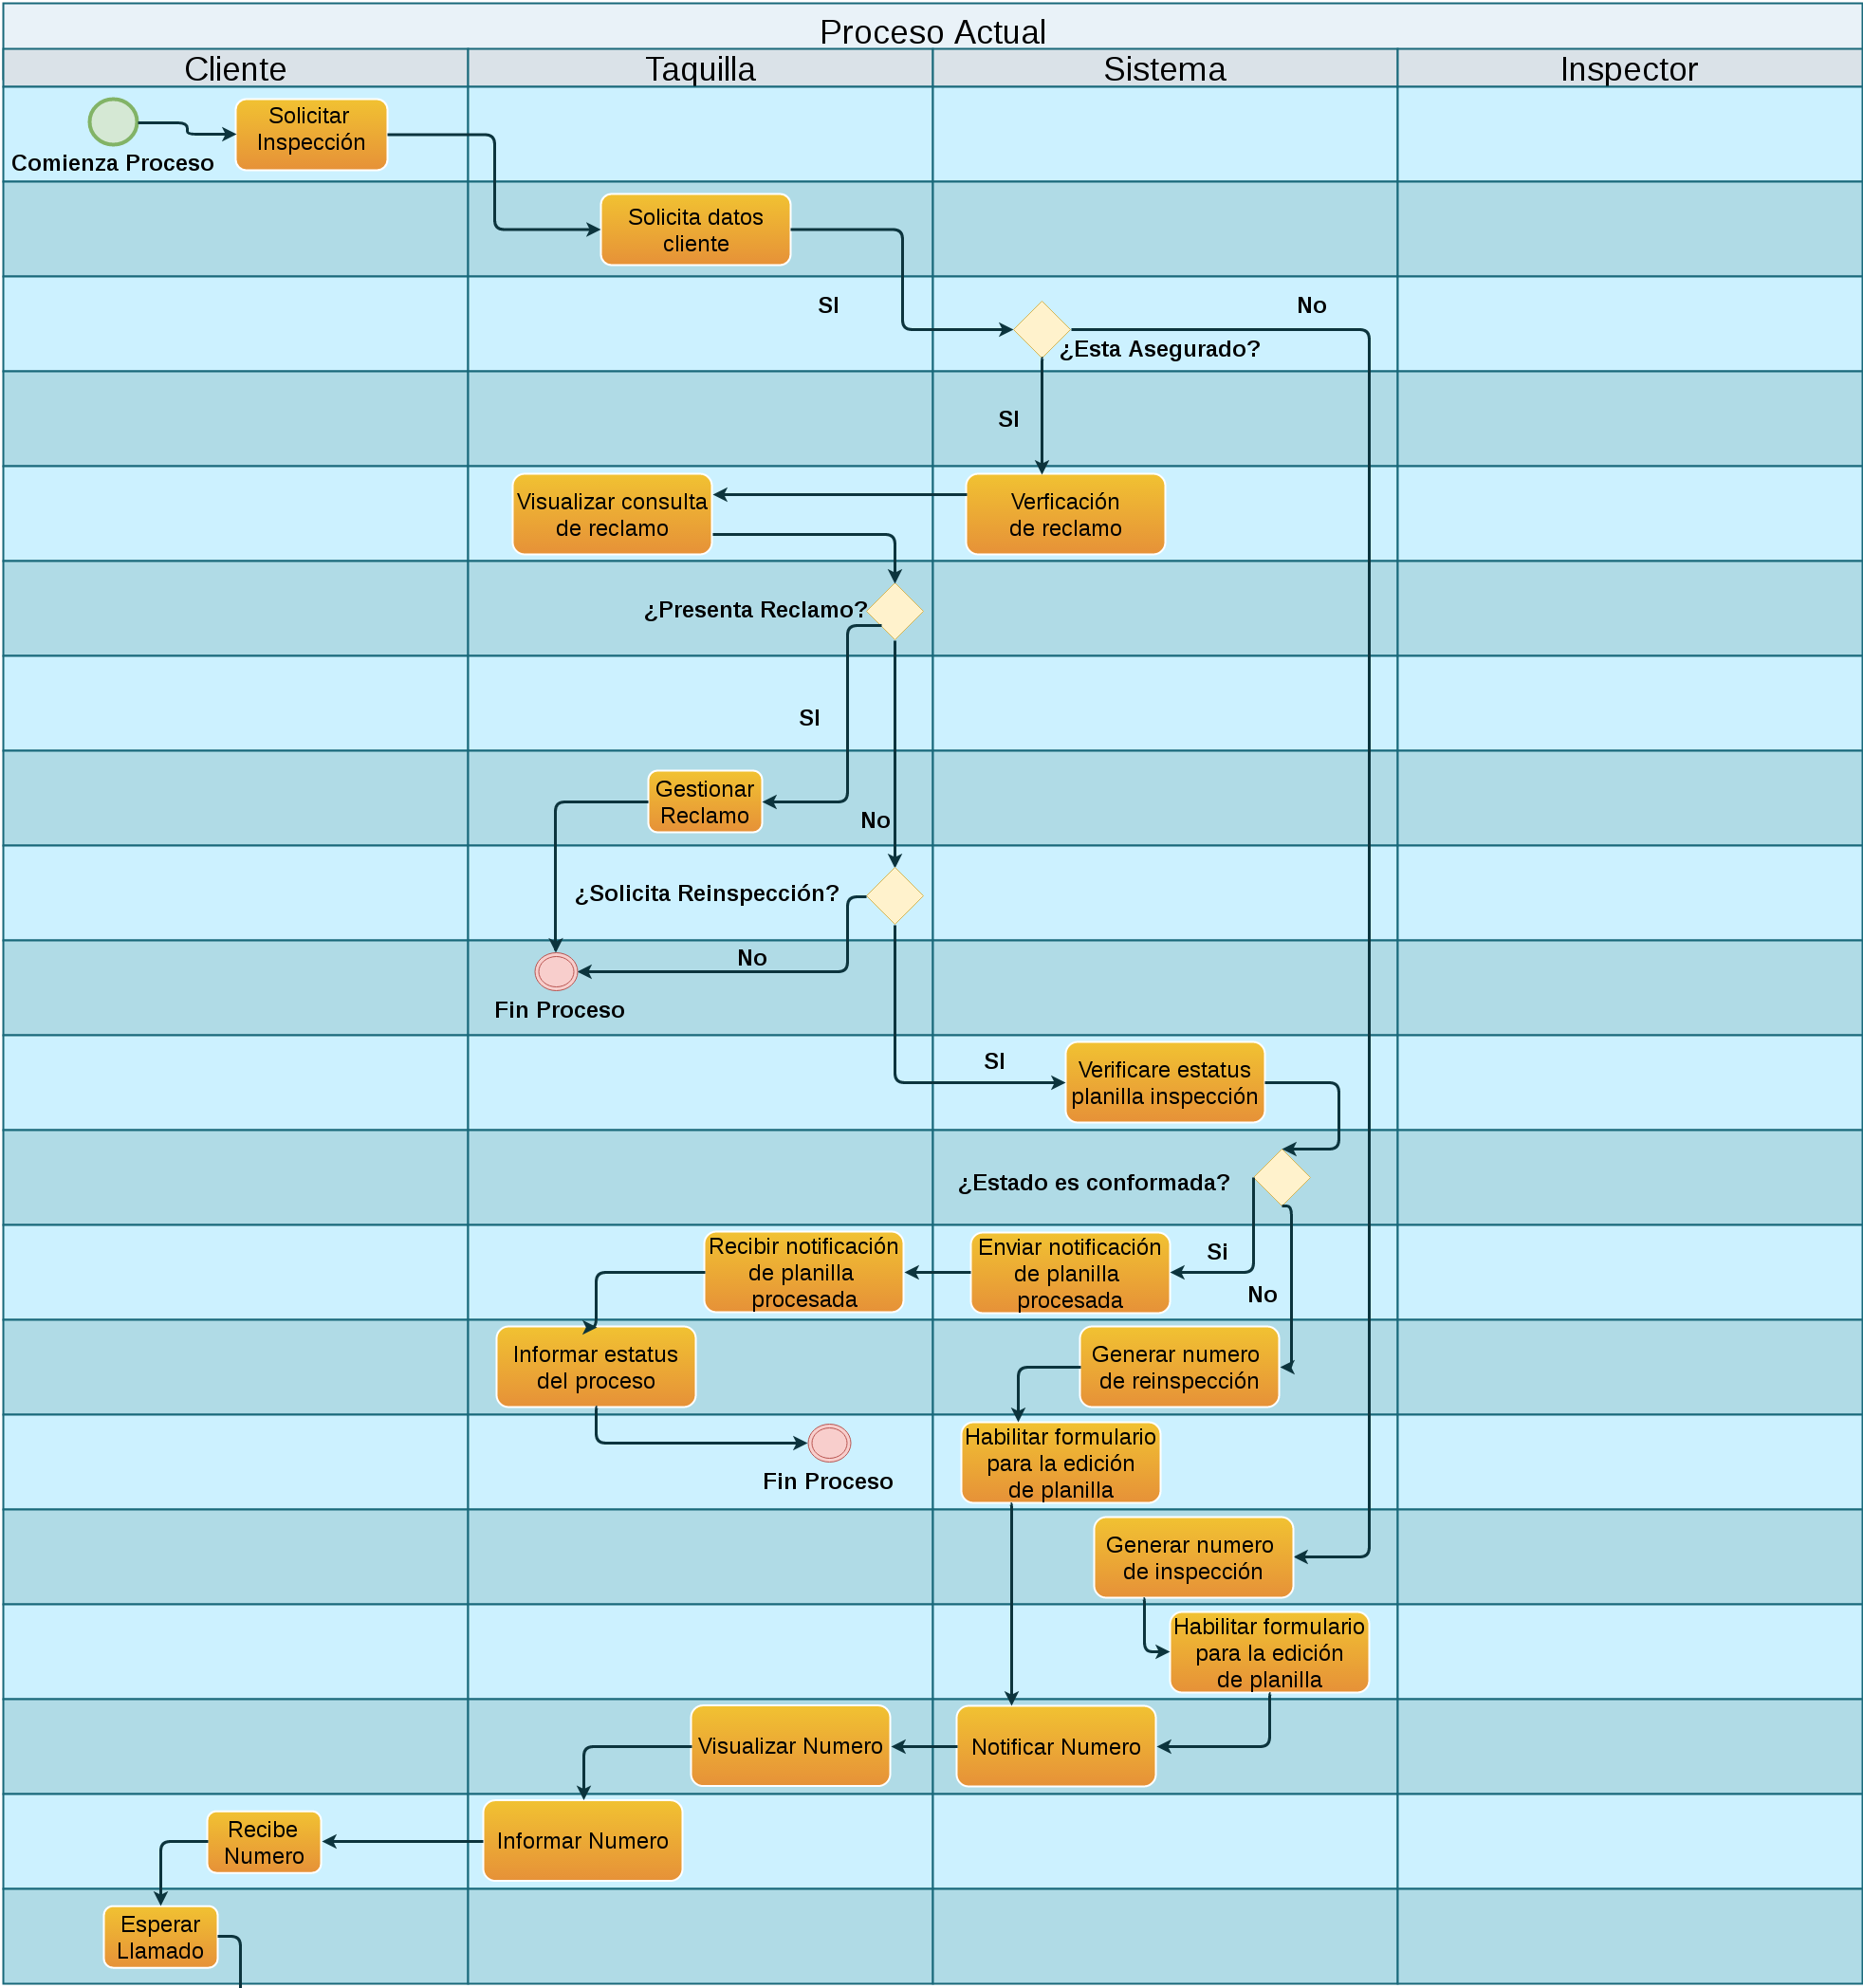
\includegraphics[width=\textwidth]{img/p1.png}
\end{center}
\caption{Flujo de la solución. (parte 1)}
\label{fig:proc_con_sistema_1}
\end{figure}

\newpage
\begin{figure}[H]
\begin{center}
	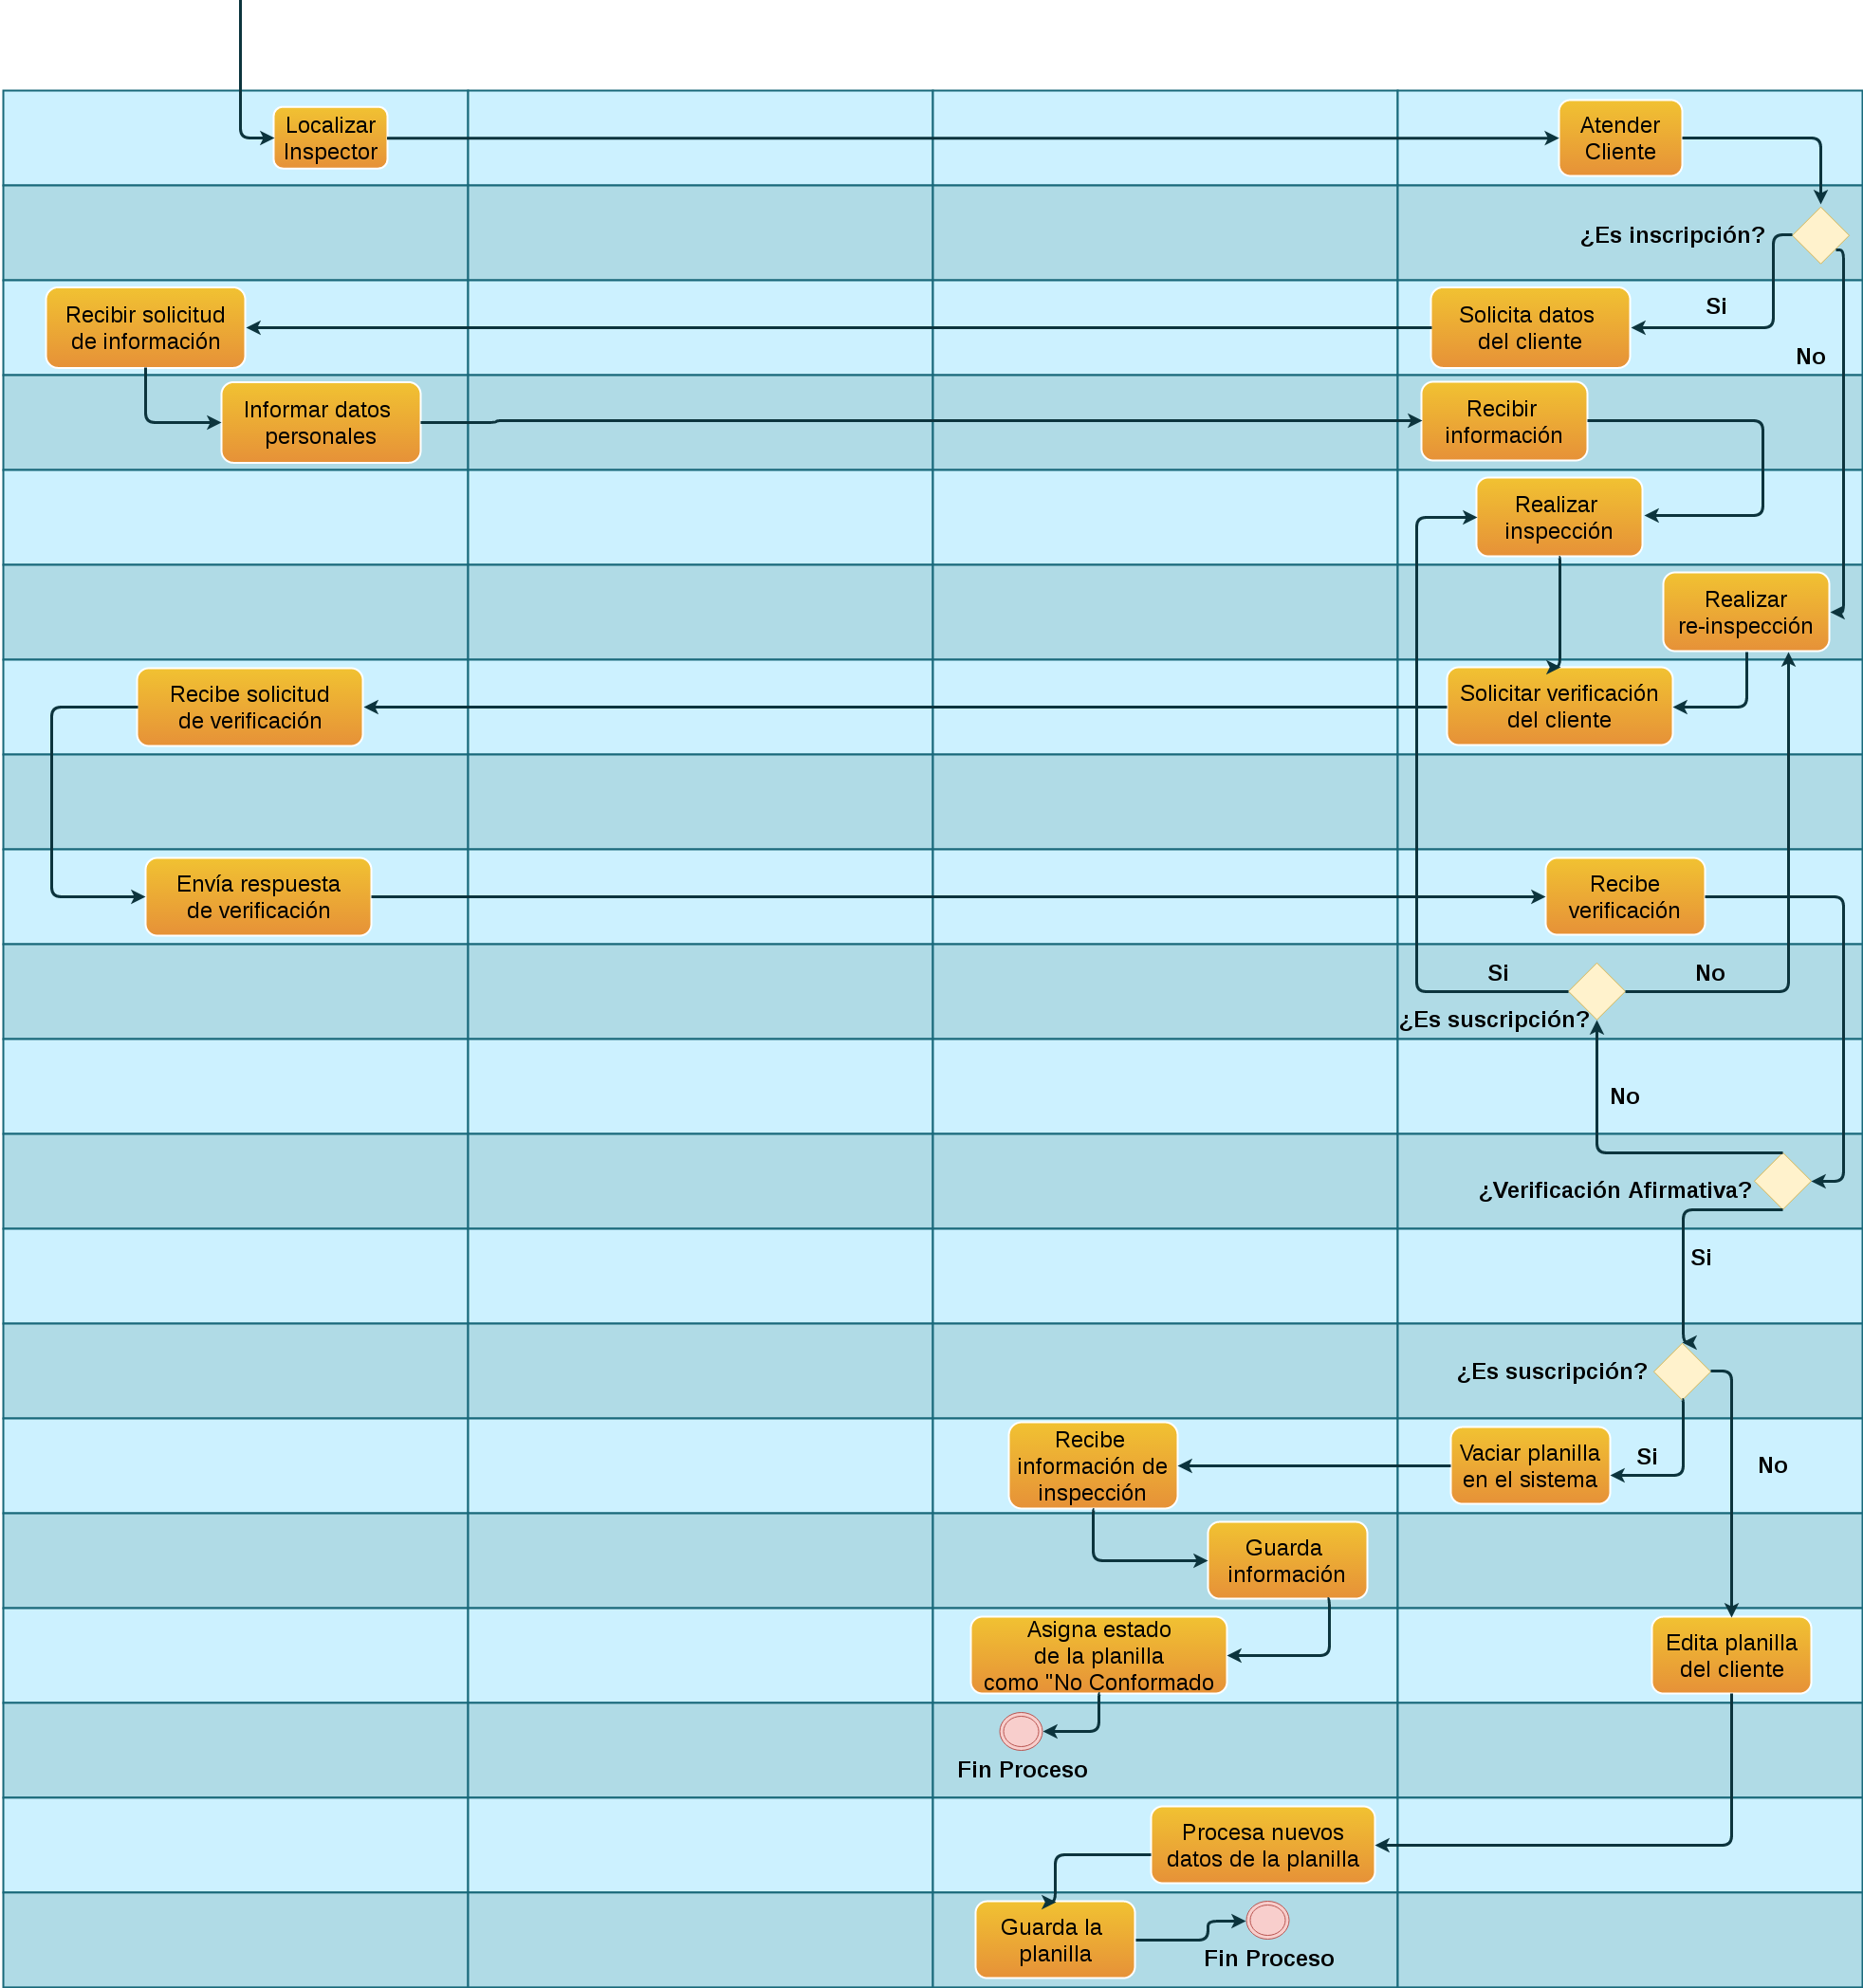
\includegraphics[width=\textwidth]{img/p2.png}
\end{center}
\caption{Flujo de la solución. (parte 2)}
\label{fig:proc_con_sistema_2}
\end{figure}

\newpage
\setlength{\parskip}{5mm}
Inicialmente, cuando un cliente desea realizar la inspección del vehículo, este deberá dirigirse a la taquilla en la cual se le identificara si esta asegurado o no, en caso de estarlo se le preguntara si quiere presentar algún reclamo o viene por una re-inspección del vehículo

En caso del reclamo, este sera manejado mediante un formulario el cual sera almacenado para posteriormente ser atendido.

En caso de que venga por una re-inspección se verificara el estatus de su planilla de suscripción del vehículo, si esta ya fue procesada se le notificara que no es posible realizar la re-inspección, ya que su solicitud de suscripción ya fue gestionada. Si la planilla de suscripción aun no ha sido aprobada se le generara un numero de re-inspección y se habilitara el formulario de edición de la planilla de suscripción asociada a ese cliente. El cliente esperara el llamado del perito el cual realizara la re-inspección del vehículo. Cuando la re-inspección termine este le pedirá la confirmación al cliente, si esta de acuerdo con los datos finales de la inspección, de ser así firmara los documentos en caso contrario se realizara nuevamente la re-inspección donde el cliente crea necesario que hay que tener especial atención. Luego el perito editara la planilla del cliente, se procesaran los nuevos datos y la planilla se guardara.

En caso de que no este registrado, el cliente recibirá un numero y tendrá que espera un tiempo, se encontrara con el perito el cual le pedirá los datos personales y comenzara a realizar la inspección, al finalizar la misma se le pedirá la verificación al cliente.

Cuando el cliente verifique que los datos son correctos el perito procederá a realizar un vaciado de la información de inspección en el formulario del sistema el cual generara la planilla de suscripción con estado "No Conformado", el cual denota que puede ser editada una vez mas antes de ser guardada definitivamente.
\setlength{\parskip}{0mm}


\newpage
\section{Alcance}

Como alcance del trabajo especial de grado se tiene previsto lograr el registro de usuarios que accederán al sistema para gestionar las planillas, la captura de los datos de la planilla de inspección, la edición de la planilla en caso de incongruencias antes de ser almacenada y guardar el conjunto de datos en la base de datos para su posterior consulta


%  mejorar la administración de las planillas de inspección de los vehículos, minimizar los riesgos de perdida de información que no esta respaldada y hacer mas eficiente el acceso a la misma.

% En referencia a las planillas que se ingresaran al sistema, este permitirá su edición en caso de errores una vez antes de ser guardadas en definitivo.

%de que van a constar, registrar el usuario, parte de captura de los datos, edicion de la planilla, configuracion de tablas?, guardar los datos en base de datos

